\documentclass[12pt]{article}
\usepackage{amsmath}
\usepackage[lmargin = 0.6in, rmargin = 0.55in, tmargin = 0.5in, bmargin = 0.8in]{geometry}
\usepackage[none]{hyphenat}
\usepackage{graphicx}
\usepackage{subcaption}

\title{Assignment 3 Bonus}
\author{Aditya Vipradas\\ASU ID: 1209435588}
\begin{document}
\maketitle
From all the given mode shapes for a truss structure, the modes corresponding to rigid body motion have a zero eigenvalue. These modes are non-deformable in nature. They signify rigid body motions which can be translations in X or Y directions or rotation in the X-Y plane for a 2D structure. The zero eigenvalue modes can be extracted using the eig(K) and quiver commands in MATLAB where K is the global stiffness matrix of the truss structure. Let us assume the input parameters as L = 5 m, H = 2 m and nb = 4. As observed from the code execution, all the 24 eigenvalues are obtained in the descending order of their magnitudes. The truss structure obtained is as follows. The quiver plots that give non-deformed or rigid modes correspond to the zero eigenvalue. Thus, the mode shape quiver plots corresponding to modes 24, 23 and 22 have rigid body motions as shown below.
\begin{figure}[ht]
  \begin{minipage}[b]{0.4\textwidth}
    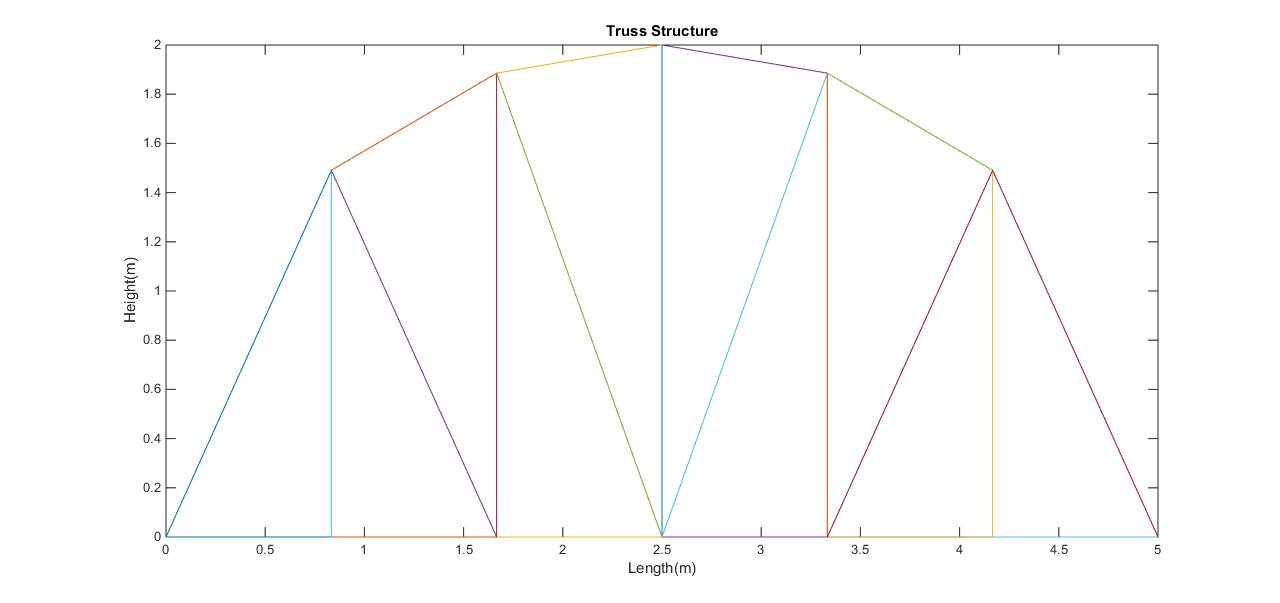
\includegraphics[scale=0.2]{truss.jpg}
  \end{minipage}
  \hfill
  \begin{minipage}[b]{0.5\textwidth}
    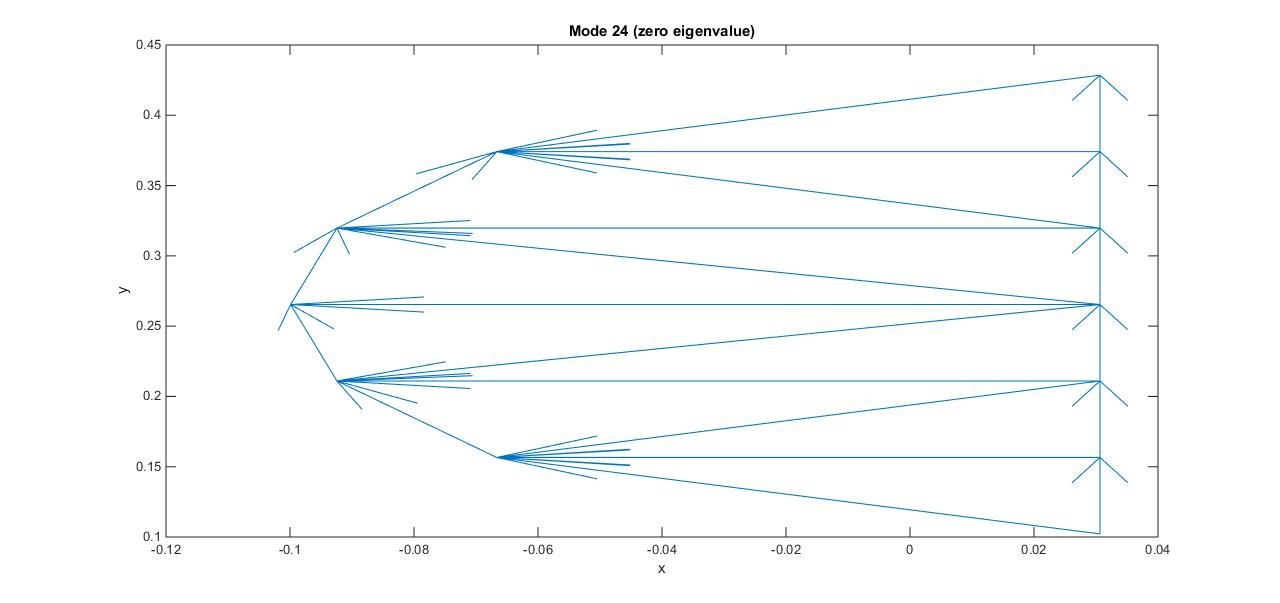
\includegraphics[scale=0.2]{mode24.jpg}
  \end{minipage}
\end{figure}
\begin{figure}[ht]
  \begin{minipage}[b]{0.4\textwidth}
    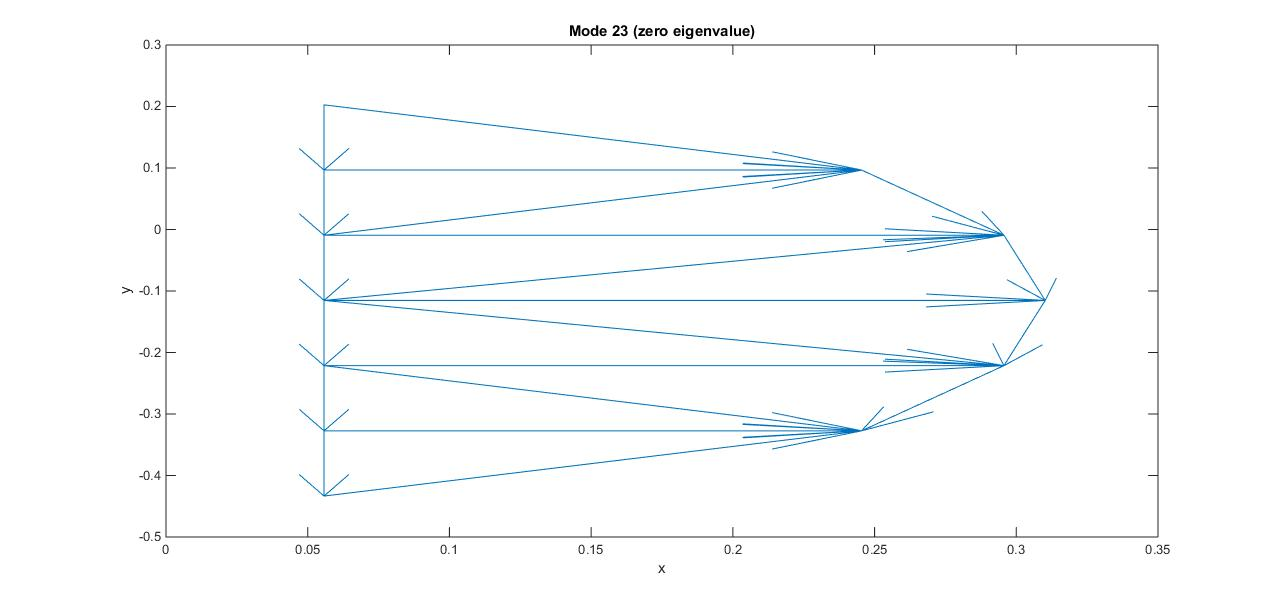
\includegraphics[scale=0.2]{mode23.jpg}
  \end{minipage}
  \hfill
  \begin{minipage}[b]{0.5\textwidth}
    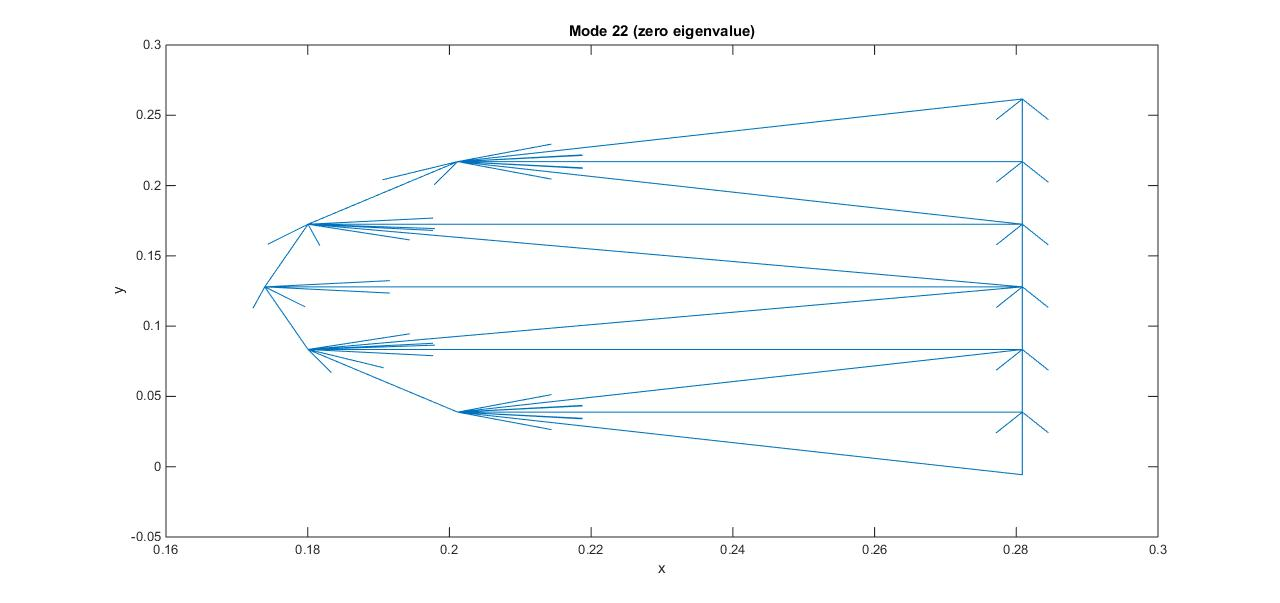
\includegraphics[scale=0.2]{mode22.jpg}
  \end{minipage}
\end{figure}
As seen, these mode shapes are obtained by rotating the given truss structure in the X-Y plane. If the eigenvalue matrix is observed, the entries at (22,22), (23,23) and (24,24) are 0.0000. The quiver plots for the remaining mode shapes from 1 to 21 are deformable and their corresponding eigenvalues are non-zero. Therefore, when the eigenvalues are non-zero, the mode shapes are deformable whereas, when the eigenvalues are zero, the mode shapes are rigid.
\end{document}